\chapter{Computed Tomography (CT)}
\label{ch:computed_tomography}

% Chapter-opening illustrated modality infographic.
\begin{center}
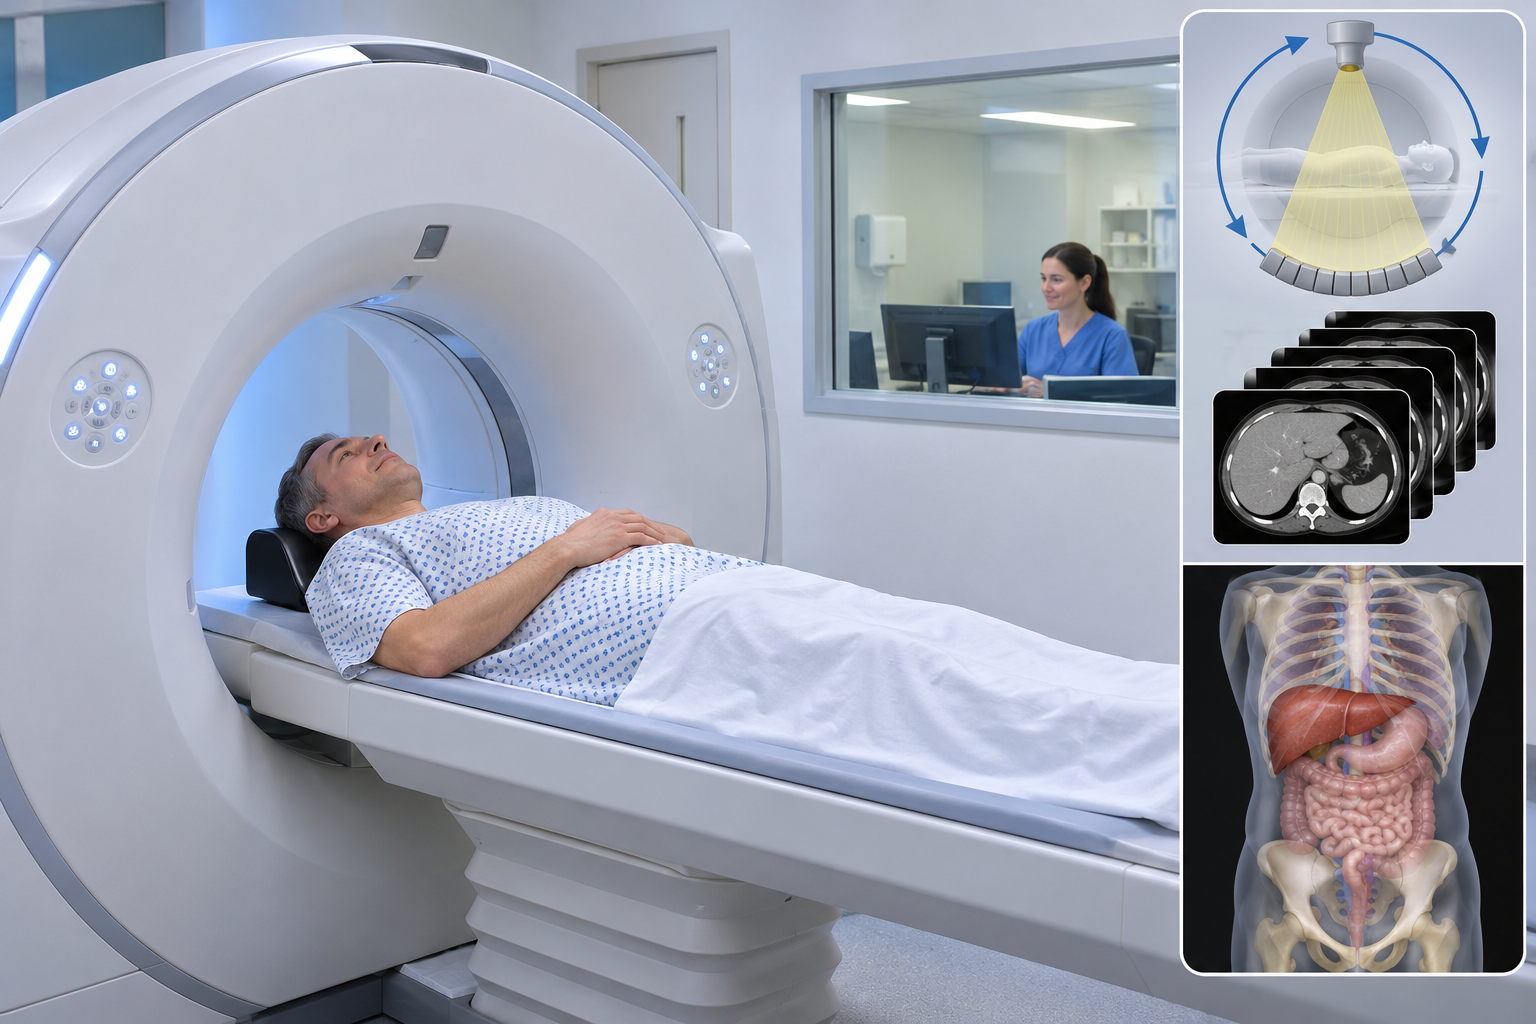
\includegraphics[width=\textwidth,keepaspectratio]{modalities/infographics/computed_tomography_realistic.png}
\end{center}
\begin{center}\footnotesize CT measures X-ray attenuation from many angles and reconstructs cross-sectional images; protocol and contrast phase shape the findings. AI-generated illustration; CT panels are not patient studies.\end{center}

\section{Overview}
Computed tomography (CT) is a cross-sectional imaging technique that uses X-rays and computational reconstruction to visualize internal anatomical structures. CT is particularly valuable for detecting tumors, hemorrhage, fractures, infections, vascular abnormalities, and traumatic injuries.

This catalogue focuses on diseases and conditions for which CT has established clinical diagnostic utility. It includes noncontrast CT, contrast-enhanced CT, high-resolution CT (HRCT), CT angiography (CTA), CT urography, and other specialized CT protocols. It excludes PET-CT and purely interventional applications.

The 312 entries form a preliminary clinical catalogue of diseases, anatomical abnormalities, and radiological findings. Some entries overlap, and not all warrant CT as a first-line investigation. Individual guideline validation is required before using these entries as diagnostic ground truth.

\section{Where CT is used}
The following numbered entries present common diagnostic applications by anatomical system. Findings are examples and should be interpreted with the clinical presentation, acquisition protocol, contrast phase, and reconstruction settings.

\subsection{Brain and intracranial structures}
\begin{enumerate}[leftmargin=*,itemsep=0.45em,topsep=0.4em]
\item \textbf{Acute ischemic stroke.} Useful imaging findings include: Early noncontrast CT may be normal; subtle loss of gray-white differentiation or hypoattenuation may develop.
\item \textbf{Arachnoid cyst.} Useful imaging findings include: Extra-axial fluid-density collection.
\item \textbf{Astrocytoma.} Useful imaging findings include: Intra-axial mass with variable enhancement.
\item \textbf{Brain metastases.} Useful imaging findings include: Enhancing lesions with surrounding edema.
\item \textbf{Cerebral abscess.} Useful imaging findings include: Ring-enhancing lesion with surrounding edema.
\item \textbf{Cerebral atrophy.} Useful imaging findings include: Enlarged sulci and ventricles.
\item \textbf{Cerebral contusion.} Useful imaging findings include: Hemorrhagic parenchymal lesions.
\item \textbf{Cerebral edema.} Useful imaging findings include: Reduced attenuation, sulcal effacement.
\item \textbf{Cerebral herniation.} Useful imaging findings include: Displacement of intracranial structures.
\item \textbf{Cerebral venous sinus thrombosis.} Useful imaging findings include: Venous filling defect on CT venography.
\item \textbf{Craniopharyngioma.} Useful imaging findings include: Cystic or solid suprasellar mass, often calcified.
\item \textbf{Epidural hematoma.} Useful imaging findings include: Biconvex extra-axial collection.
\item \textbf{Glioblastoma.} Useful imaging findings include: Irregular enhancing mass with central necrosis.
\item \textbf{Hydrocephalus.} Useful imaging findings include: Ventricular enlargement.
\item \textbf{Intracerebral hemorrhage.} Useful imaging findings include: Hyperdense intraparenchymal blood.
\item \textbf{Intracranial tuberculoma.} Useful imaging findings include: Nodular or ring-enhancing lesions.
\item \textbf{Intraventricular hemorrhage.} Useful imaging findings include: Hyperdense blood within ventricles.
\item \textbf{Meningioma.} Useful imaging findings include: Enhancing extra-axial mass.
\item \textbf{Neurocysticercosis.} Useful imaging findings include: Cystic lesions or intracranial calcifications.
\item \textbf{Oligodendroglioma.} Useful imaging findings include: Intra-axial mass with possible calcifications.
\item \textbf{Pituitary macroadenoma.} Useful imaging findings include: Enlarged sellar or suprasellar mass.
\item \textbf{Pneumocephalus.} Useful imaging findings include: Intracranial air.
\item \textbf{Subarachnoid hemorrhage.} Useful imaging findings include: Hyperdensity within cerebral sulci and cisterns.
\item \textbf{Subdural hematoma.} Useful imaging findings include: Crescent-shaped extra-axial collection.
\end{enumerate}

\subsection{Head, neck and facial structures}
\begin{enumerate}[leftmargin=*,itemsep=0.45em,topsep=0.4em]
\item \textbf{Acute sinusitis.} Useful imaging findings include: Mucosal thickening or fluid may be seen but is nonspecific; CT is not indicated for uncomplicated disease.
\item \textbf{Branchial cleft cyst.} Useful imaging findings include: Lateral cervical cystic lesion.
\item \textbf{Cervical lymphadenopathy.} Useful imaging findings include: Enlarged or necrotic cervical lymph nodes.
\item \textbf{Cholesteatoma.} Useful imaging findings include: Middle-ear soft tissue with bony erosion.
\item \textbf{Chronic sinusitis.} Useful imaging findings include: Mucosal thickening, bony remodeling.
\item \textbf{Invasive fungal sinusitis.} Useful imaging findings include: Extrasinus infiltration, possible bone destruction.
\item \textbf{Laryngeal carcinoma.} Useful imaging findings include: Laryngeal mass with possible cartilage invasion.
\item \textbf{Ludwig angina.} Useful imaging findings include: Floor-of-mouth inflammatory changes.
\item \textbf{Mastoiditis.} Useful imaging findings include: Mastoid opacification, possible septal erosion.
\item \textbf{Nasal polyposis.} Useful imaging findings include: Polypoid sinonasal soft tissue.
\item \textbf{Nasopharyngeal carcinoma.} Useful imaging findings include: Nasopharyngeal soft-tissue mass.
\item \textbf{Orbital abscess.} Useful imaging findings include: Rim-enhancing orbital collection.
\item \textbf{Orbital cellulitis.} Useful imaging findings include: Orbital fat stranding.
\item \textbf{Orbital fracture.} Useful imaging findings include: Discontinuity of orbital walls.
\item \textbf{Otosclerosis.} Useful imaging findings include: Abnormal otic capsule mineralization.
\item \textbf{Parotid tumor.} Useful imaging findings include: Focal parotid mass.
\item \textbf{Peritonsillar abscess.} Useful imaging findings include: Peritonsillar fluid collection.
\item \textbf{Retropharyngeal abscess.} Useful imaging findings include: Rim-enhancing retropharyngeal collection.
\item \textbf{Sialolithiasis.} Useful imaging findings include: Calcified salivary duct stone.
\item \textbf{Sinus mucocele.} Useful imaging findings include: Expansile opacified sinus.
\item \textbf{Thyroglossal duct cyst.} Useful imaging findings include: Midline cervical cystic lesion.
\item \textbf{Thyroid eye disease.} Useful imaging findings include: Extraocular muscle enlargement.
\end{enumerate}

CT findings of mastoid opacification alone are not specific for acute mastoiditis; bony erosion and clinical evidence of complication increase concern.

\subsection{Pulmonary and thoracic diseases}
\begin{enumerate}[leftmargin=*,itemsep=0.45em,topsep=0.4em]
\item \textbf{Allergic bronchopulmonary aspergillosis.} Useful imaging findings include: Central bronchiectasis and mucus plugging.
\item \textbf{ARDS.} Useful imaging findings include: Bilateral ground-glass opacities and consolidation.
\item \textbf{Asbestosis.} Useful imaging findings include: Subpleural fibrosis, pleural plaques.
\item \textbf{Atelectasis.} Useful imaging findings include: Pulmonary volume loss.
\item \textbf{Bronchiectasis.} Useful imaging findings include: Bronchial dilatation, signet-ring sign.
\item \textbf{Diaphragmatic hernia.} Useful imaging findings include: Abdominal contents within the thorax.
\item \textbf{Empyema.} Useful imaging findings include: Loculated pleural fluid, split-pleura sign.
\item \textbf{Hemothorax.} Useful imaging findings include: High-attenuation pleural fluid.
\item \textbf{Hypersensitivity pneumonitis.} Useful imaging findings include: Mosaic attenuation, centrilobular nodules.
\item \textbf{Idiopathic pulmonary fibrosis.} Useful imaging findings include: Subpleural basal fibrosis and honeycombing.
\item \textbf{Lung abscess.} Useful imaging findings include: Cavitary lesion with air-fluid level.
\item \textbf{Lung carcinoma.} Useful imaging findings include: Pulmonary nodule or mass.
\item \textbf{Lymphangioleiomyomatosis.} Useful imaging findings include: Multiple thin-walled pulmonary cysts.
\item \textbf{Lymphangitic carcinomatosis.} Useful imaging findings include: Nodular interlobular septal thickening.
\item \textbf{Nonspecific interstitial pneumonia.} Useful imaging findings include: Ground-glass opacities and fine reticulation.
\item \textbf{Organizing pneumonia.} Useful imaging findings include: Peripheral or peribronchovascular consolidation.
\item \textbf{Pleural effusion.} Useful imaging findings include: Pleural fluid collection.
\item \textbf{Pleural mesothelioma.} Useful imaging findings include: Nodular pleural thickening.
\item \textbf{Pneumonia.} Useful imaging findings include: Consolidation, ground-glass opacities.
\item \textbf{Pneumothorax.} Useful imaging findings include: Pleural air.
\item \textbf{Pulmonary alveolar proteinosis.} Useful imaging findings include: Crazy-paving pattern.
\item \textbf{Pulmonary aspergilloma.} Useful imaging findings include: Intracavitary fungal mass.
\item \textbf{Pulmonary edema.} Useful imaging findings include: Septal thickening, ground-glass opacities.
\item \textbf{Pulmonary embolism.} Useful imaging findings include: Pulmonary arterial filling defect.
\item \textbf{Pulmonary emphysema.} Useful imaging findings include: Low-attenuation lung regions.
\item \textbf{Pulmonary fibrosis.} Useful imaging findings include: Reticulation, architectural distortion.
\item \textbf{Pulmonary hamartoma.} Useful imaging findings include: Fat-containing nodule, possible popcorn calcification.
\item \textbf{Pulmonary infarction.} Useful imaging findings include: Peripheral wedge-shaped opacity.
\item \textbf{Pulmonary Langerhans cell histiocytosis.} Useful imaging findings include: Upper-lobe nodules and irregular cysts.
\item \textbf{Pulmonary metastases.} Useful imaging findings include: Single or multiple pulmonary nodules.
\item \textbf{Pulmonary sarcoidosis.} Useful imaging findings include: Perilymphatic nodules, hilar lymphadenopathy.
\item \textbf{Pulmonary sequestration.} Useful imaging findings include: Abnormal lung tissue with systemic arterial supply.
\item \textbf{Pulmonary tuberculosis.} Useful imaging findings include: Cavitation, tree-in-bud nodules.
\item \textbf{Silicosis.} Useful imaging findings include: Upper-lobe nodules, possible eggshell calcification.
\item \textbf{Tracheomalacia.} Useful imaging findings include: Expiratory tracheal collapse.
\end{enumerate}

For suspected pulmonary fibrosis, high-resolution CT (HRCT) is the relevant protocol; these patterns are not specific to a single cause.

\subsection{Heart and mediastinum}
\begin{enumerate}[leftmargin=*,itemsep=0.45em,topsep=0.4em]
\item \textbf{Anomalous coronary artery.} Useful imaging findings include: Abnormal coronary origin or course.
\item \textbf{Bronchogenic cyst.} Useful imaging findings include: Mediastinal cystic lesion.
\item \textbf{Constrictive pericarditis.} Useful imaging findings include: Pericardial thickening or calcification.
\item \textbf{Coronary artery aneurysm.} Useful imaging findings include: Focal coronary arterial dilatation.
\item \textbf{Coronary artery calcification.} Useful imaging findings include: Calcified coronary atherosclerotic plaques.
\item \textbf{Coronary artery disease.} Useful imaging findings include: Coronary plaque and luminal stenosis.
\item \textbf{Fibrosing mediastinitis.} Useful imaging findings include: Infiltrative mediastinal fibrosis.
\item \textbf{Left atrial appendage thrombus.} Useful imaging findings include: Persistent intracavitary filling defect.
\item \textbf{Left ventricular aneurysm.} Useful imaging findings include: Ventricular outpouching.
\item \textbf{Mediastinal lymphoma.} Useful imaging findings include: Mediastinal soft-tissue masses or lymphadenopathy.
\item \textbf{Mediastinal teratoma.} Useful imaging findings include: Mixed fat, fluid, and calcified components.
\item \textbf{Mediastinitis.} Useful imaging findings include: Mediastinal inflammatory changes.
\item \textbf{Myocardial bridging.} Useful imaging findings include: Intramyocardial coronary artery segment.
\item \textbf{Pericardial cyst.} Useful imaging findings include: Well-defined fluid-density lesion.
\item \textbf{Pericardial effusion.} Useful imaging findings include: Pericardial fluid.
\item \textbf{Pneumomediastinum.} Useful imaging findings include: Extraluminal mediastinal air.
\item \textbf{Thymic hyperplasia.} Useful imaging findings include: Enlarged thymic tissue.
\item \textbf{Thymoma.} Useful imaging findings include: Anterior mediastinal mass.
\end{enumerate}

\subsection{Liver}
\begin{enumerate}[leftmargin=*,itemsep=0.45em,topsep=0.4em]
\item \textbf{Budd--Chiari syndrome.} Useful imaging findings include: Hepatic venous obstruction and heterogeneous enhancement.
\item \textbf{Congestive hepatopathy.} Useful imaging findings include: Heterogeneous enhancement and dilated hepatic veins.
\item \textbf{Focal nodular hyperplasia.} Useful imaging findings include: Arterial hyperenhancement, possible central scar.
\item \textbf{Hepatic adenoma.} Useful imaging findings include: Hypervascular mass with variable fat or hemorrhage.
\item \textbf{Hepatic hemangioma.} Useful imaging findings include: Peripheral nodular enhancement with progressive fill-in.
\item \textbf{Hepatic hematoma.} Useful imaging findings include: Blood collection within or adjacent to the liver.
\item \textbf{Hepatic infarction.} Useful imaging findings include: Peripheral wedge-shaped hypoenhancement.
\item \textbf{Hepatic metastases.} Useful imaging findings include: Focal lesions with variable enhancement.
\item \textbf{Hepatic steatosis.} Useful imaging findings include: Reduced hepatic attenuation.
\item \textbf{Hepatocellular carcinoma.} Useful imaging findings include: Arterial hyperenhancement and subsequent washout.
\item \textbf{Hepatomegaly.} Useful imaging findings include: Increased liver dimensions.
\item \textbf{Hydatid disease.} Useful imaging findings include: Daughter cysts and possible wall calcification.
\item \textbf{Intrahepatic cholangiocarcinoma.} Useful imaging findings include: Mass with progressive delayed enhancement.
\item \textbf{Liver abscess.} Useful imaging findings include: Rim-enhancing fluid collection.
\item \textbf{Liver cirrhosis.} Useful imaging findings include: Nodular contour and altered hepatic morphology.
\item \textbf{Polycystic liver disease.} Useful imaging findings include: Multiple hepatic cysts.
\item \textbf{Portal hypertension.} Useful imaging findings include: Portosystemic collateral vessels, splenomegaly.
\item \textbf{Simple hepatic cyst.} Useful imaging findings include: Nonenhancing fluid-density lesion.
\end{enumerate}

\subsection{Gallbladder and biliary system}
\begin{enumerate}[leftmargin=*,itemsep=0.45em,topsep=0.4em]
\item \textbf{Acute cholecystitis.} Useful imaging findings include: Gallbladder wall thickening and surrounding inflammation; ultrasound is generally first-line.
\item \textbf{Biliary obstruction.} Useful imaging findings include: Bile duct dilatation.
\item \textbf{Cholangiocarcinoma.} Useful imaging findings include: Biliary mass or irregular ductal narrowing.
\item \textbf{Choledochal cyst.} Useful imaging findings include: Cystic biliary dilatation.
\item \textbf{Choledocholithiasis.} Useful imaging findings include: Visible common bile duct calculus.
\item \textbf{Cholelithiasis.} Useful imaging findings include: Some calcified or otherwise conspicuous stones; CT may miss noncalcified stones, and ultrasound is generally first-line.
\item \textbf{Emphysematous cholecystitis.} Useful imaging findings include: Gas within the gallbladder wall or lumen.
\item \textbf{Gallbladder carcinoma.} Useful imaging findings include: Irregular enhancing mass.
\item \textbf{Gallbladder perforation.} Useful imaging findings include: Focal wall defect and adjacent fluid.
\item \textbf{Gangrenous cholecystitis.} Useful imaging findings include: Irregular or absent mural enhancement.
\item \textbf{Porcelain gallbladder.} Useful imaging findings include: Gallbladder wall calcification.
\end{enumerate}

Ultrasound is generally preferred for the initial assessment of suspected gallstones and uncomplicated acute cholecystitis.

\subsection{Pancreas}
\begin{enumerate}[leftmargin=*,itemsep=0.45em,topsep=0.4em]
\item \textbf{Acute pancreatitis.} Useful imaging findings include: Pancreatic enlargement and surrounding inflammation.
\item \textbf{Autoimmune pancreatitis.} Useful imaging findings include: Diffuse sausage-shaped pancreatic enlargement.
\item \textbf{Chronic pancreatitis.} Useful imaging findings include: Calcifications, ductal dilatation, atrophy.
\item \textbf{Intraductal papillary mucinous neoplasm.} Useful imaging findings include: Pancreatic duct dilatation or communicating cysts.
\item \textbf{Mucinous cystic neoplasm.} Useful imaging findings include: Cystic lesion with septations.
\item \textbf{Necrotizing pancreatitis.} Useful imaging findings include: Nonenhancing pancreatic or peripancreatic tissue.
\item \textbf{Pancreatic adenocarcinoma.} Useful imaging findings include: Hypoenhancing pancreatic mass.
\item \textbf{Pancreatic duct obstruction.} Useful imaging findings include: Upstream pancreatic duct dilatation.
\item \textbf{Pancreatic neuroendocrine tumor.} Useful imaging findings include: Typically hypervascular pancreatic lesion.
\item \textbf{Pancreatic pseudocyst.} Useful imaging findings include: Encapsulated homogeneous fluid collection.
\item \textbf{Serous cystadenoma.} Useful imaging findings include: Multicystic lesion, possible central scar.
\item \textbf{Solid pseudopapillary neoplasm.} Useful imaging findings include: Encapsulated solid-cystic mass.
\item \textbf{Walled-off pancreatic necrosis.} Useful imaging findings include: Encapsulated collection containing necrotic material.
\end{enumerate}

\subsection{Spleen}
\begin{enumerate}[leftmargin=*,itemsep=0.45em,topsep=0.4em]
\item \textbf{Splenic abscess.} Useful imaging findings include: Low-attenuation lesion with possible rim enhancement.
\item \textbf{Splenic cyst.} Useful imaging findings include: Fluid-density lesion.
\item \textbf{Splenic hemangioma.} Useful imaging findings include: Vascular lesion with variable enhancement.
\item \textbf{Splenic hematoma.} Useful imaging findings include: Intraparenchymal or subcapsular blood collection.
\item \textbf{Splenic infarction.} Useful imaging findings include: Peripheral wedge-shaped hypoattenuation.
\item \textbf{Splenic lymphoma.} Useful imaging findings include: Splenomegaly or focal lesions.
\item \textbf{Splenic rupture.} Useful imaging findings include: Parenchymal disruption and hemorrhage.
\item \textbf{Splenic torsion.} Useful imaging findings include: Twisted vascular pedicle and impaired enhancement.
\item \textbf{Splenomegaly.} Useful imaging findings include: Enlarged spleen.
\item \textbf{Wandering spleen.} Useful imaging findings include: Abnormal splenic location.
\end{enumerate}

\subsection{Gastrointestinal system}
\begin{enumerate}[leftmargin=*,itemsep=0.45em,topsep=0.4em]
\item \textbf{Abdominal hernia.} Useful imaging findings include: Protrusion through an abdominal wall defect.
\item \textbf{Acute appendicitis.} Useful imaging findings include: Enlarged appendix with surrounding inflammation.
\item \textbf{Appendiceal abscess.} Useful imaging findings include: Localized rim-enhancing collection.
\item \textbf{Cecal volvulus.} Useful imaging findings include: Displaced dilated cecum with mesenteric twisting.
\item \textbf{Colorectal carcinoma.} Useful imaging findings include: Focal irregular bowel wall thickening.
\item \textbf{Crohn disease.} Useful imaging findings include: Bowel wall thickening, hyperenhancement, comb sign.
\item \textbf{Diverticulitis.} Useful imaging findings include: Inflamed diverticula and pericolic fat stranding.
\item \textbf{Epiploic appendagitis.} Useful imaging findings include: Oval fat-density lesion with hyperattenuating rim.
\item \textbf{Esophageal carcinoma.} Useful imaging findings include: Esophageal wall thickening or mass.
\item \textbf{Gastric carcinoma.} Useful imaging findings include: Irregular gastric wall thickening or mass.
\item \textbf{Gastric volvulus.} Useful imaging findings include: Abnormal gastric rotation.
\item \textbf{Gastrointestinal perforation.} Useful imaging findings include: Extraluminal gas.
\item \textbf{Gastrointestinal stromal tumor.} Useful imaging findings include: Exophytic enhancing gastrointestinal mass.
\item \textbf{Infectious colitis.} Useful imaging findings include: Colonic wall thickening and mucosal enhancement.
\item \textbf{Internal hernia.} Useful imaging findings include: Abnormally positioned bowel loops and mesenteric vessels.
\item \textbf{Intestinal malrotation.} Useful imaging findings include: Abnormal bowel and mesenteric vascular arrangement.
\item \textbf{Intussusception.} Useful imaging findings include: Bowel-within-bowel configuration.
\item \textbf{Ischemic colitis.} Useful imaging findings include: Segmental wall thickening and altered enhancement.
\item \textbf{Large bowel obstruction.} Useful imaging findings include: Proximal colonic dilatation.
\item \textbf{Meckel diverticulitis.} Useful imaging findings include: Inflamed blind-ending bowel structure.
\item \textbf{Mesenteric ischemia.} Useful imaging findings include: Abnormal bowel enhancement, vascular obstruction.
\item \textbf{Omental infarction.} Useful imaging findings include: Focal inflammatory fatty lesion.
\item \textbf{Paralytic ileus.} Useful imaging findings include: Diffuse bowel dilatation without mechanical obstruction.
\item \textbf{Pneumatosis intestinalis.} Useful imaging findings include: Gas within the bowel wall.
\item \textbf{Portal venous gas.} Useful imaging findings include: Peripheral branching hepatic gas.
\item \textbf{Pseudomembranous colitis.} Useful imaging findings include: Marked colonic wall thickening.
\item \textbf{Sigmoid volvulus.} Useful imaging findings include: Twisted mesentery and dilated sigmoid colon.
\item \textbf{Small bowel lymphoma.} Useful imaging findings include: Bowel wall thickening, sometimes aneurysmal dilatation.
\item \textbf{Small bowel obstruction.} Useful imaging findings include: Dilated bowel loops with transition point.
\item \textbf{Stercoral colitis.} Useful imaging findings include: Fecal impaction with surrounding inflammation.
\item \textbf{Superior mesenteric artery syndrome.} Useful imaging findings include: Duodenal compression between the aorta and SMA.
\item \textbf{Toxic megacolon.} Useful imaging findings include: Marked colonic dilatation.
\item \textbf{Ulcerative colitis.} Useful imaging findings include: Continuous colonic wall thickening.
\end{enumerate}

\subsection{Kidneys and urinary tract}
\begin{enumerate}[leftmargin=*,itemsep=0.45em,topsep=0.4em]
\item \textbf{Acute pyelonephritis.} Useful imaging findings include: Striated nephrogram or wedge-shaped hypoenhancement in selected complicated cases; routine imaging is unnecessary for uncomplicated first presentations.
\item \textbf{Bladder carcinoma.} Useful imaging findings include: Focal bladder wall mass.
\item \textbf{Bladder stones.} Useful imaging findings include: Intraluminal calculi.
\item \textbf{Complex renal cyst.} Useful imaging findings include: Septations, thickened walls, or enhancing components.
\item \textbf{Emphysematous cystitis.} Useful imaging findings include: Gas within the bladder wall.
\item \textbf{Emphysematous pyelonephritis.} Useful imaging findings include: Gas within renal tissue or surrounding spaces.
\item \textbf{Horseshoe kidney.} Useful imaging findings include: Fusion of renal poles.
\item \textbf{Hydronephrosis.} Useful imaging findings include: Dilated renal collecting system.
\item \textbf{Hydroureter.} Useful imaging findings include: Dilated ureter.
\item \textbf{Nephrolithiasis.} Useful imaging findings include: Renal calculi.
\item \textbf{Perinephric abscess.} Useful imaging findings include: Fluid collection surrounding the kidney.
\item \textbf{Polycystic kidney disease.} Useful imaging findings include: Multiple bilateral renal cysts.
\item \textbf{Renal abscess.} Useful imaging findings include: Rim-enhancing renal collection.
\item \textbf{Renal angiomyolipoma.} Useful imaging findings include: Renal mass containing macroscopic fat.
\item \textbf{Renal atrophy.} Useful imaging findings include: Reduced renal size.
\item \textbf{Renal cell carcinoma.} Useful imaging findings include: Enhancing renal mass.
\item \textbf{Renal infarction.} Useful imaging findings include: Wedge-shaped nonenhancing renal region.
\item \textbf{Renal oncocytoma.} Useful imaging findings include: Enhancing solid renal mass; CT cannot reliably distinguish oncocytoma from renal malignancy.
\item \textbf{Renal papillary necrosis.} Useful imaging findings include: Papillary abnormalities on excretory-phase imaging.
\item \textbf{Renal tuberculosis.} Useful imaging findings include: Calyceal deformity and calcification.
\item \textbf{Retroperitoneal fibrosis.} Useful imaging findings include: Periaortic soft tissue encasing retroperitoneal structures.
\item \textbf{Simple renal cyst.} Useful imaging findings include: Nonenhancing fluid-density lesion.
\item \textbf{Staghorn calculus.} Useful imaging findings include: Branching renal collecting system calculus.
\item \textbf{Ureterolithiasis.} Useful imaging findings include: Ureteral calculi.
\item \textbf{Ureteropelvic junction obstruction.} Useful imaging findings include: Collecting system dilatation with junctional narrowing.
\item \textbf{Urinary bladder rupture.} Useful imaging findings include: Extraluminal contrast on CT cystography.
\item \textbf{Urothelial carcinoma.} Useful imaging findings include: Enhancing lesion or urinary tract filling defect.
\item \textbf{Xanthogranulomatous pyelonephritis.} Useful imaging findings include: Enlarged kidney with bear-paw appearance.
\end{enumerate}

\subsection{Adrenal glands}
\begin{enumerate}[leftmargin=*,itemsep=0.45em,topsep=0.4em]
\item \textbf{Adrenal adenoma.} Useful imaging findings include: Low unenhanced attenuation or characteristic contrast washout.
\item \textbf{Adrenal carcinoma.} Useful imaging findings include: Large heterogeneous adrenal mass.
\item \textbf{Adrenal cyst.} Useful imaging findings include: Fluid-density adrenal lesion.
\item \textbf{Adrenal hemorrhage.} Useful imaging findings include: Hyperattenuating adrenal enlargement.
\item \textbf{Adrenal hyperplasia.} Useful imaging findings include: Diffuse or nodular adrenal enlargement.
\item \textbf{Adrenal metastases.} Useful imaging findings include: Adrenal masses with variable enhancement.
\item \textbf{Adrenal myelolipoma.} Useful imaging findings include: Macroscopic fat-containing adrenal mass.
\item \textbf{Adrenal tuberculosis.} Useful imaging findings include: Adrenal enlargement or calcification.
\item \textbf{Pheochromocytoma.} Useful imaging findings include: Adrenal mass with variable enhancement.
\end{enumerate}

\subsection{Female reproductive system and pelvis}
\begin{enumerate}[leftmargin=*,itemsep=0.45em,topsep=0.4em]
\item \textbf{Cervical carcinoma.} Useful imaging findings include: Cervical mass and possible adjacent invasion.
\item \textbf{Endometrial carcinoma.} Useful imaging findings include: Endometrial mass or uterine cavity abnormality.
\item \textbf{Hydrosalpinx.} Useful imaging findings include: Dilated fluid-filled fallopian tube.
\item \textbf{Ovarian carcinoma.} Useful imaging findings include: Complex adnexal mass, possible peritoneal metastases.
\item \textbf{Ovarian cyst.} Useful imaging findings include: Fluid-density adnexal lesion.
\item \textbf{Ovarian dermoid cyst.} Useful imaging findings include: Fat-containing adnexal lesion.
\item \textbf{Ovarian torsion.} Useful imaging findings include: Enlarged ovary or twisted pedicle may be visible; ultrasound is generally first-line and CT does not exclude torsion.
\item \textbf{Ovarian vein thrombosis.} Useful imaging findings include: Venous filling defect.
\item \textbf{Pelvic congestion.} Useful imaging findings include: Dilated pelvic venous structures.
\item \textbf{Pelvic hematoma.} Useful imaging findings include: Hyperattenuating pelvic collection.
\item \textbf{Pelvic inflammatory disease.} Useful imaging findings include: Pelvic inflammatory changes.
\item \textbf{Tubo-ovarian abscess.} Useful imaging findings include: Complex rim-enhancing adnexal collection.
\item \textbf{Uterine fibroids.} Useful imaging findings include: Uterine masses with variable enhancement or calcification; ultrasound or MRI is preferred for primary characterization.
\end{enumerate}

Ultrasound and MRI are generally preferred for primary characterization of gynecological abnormalities. CT is valuable in emergencies, complications, and cancer staging.

\subsection{Blood vessels and vascular diseases}
\textbf{Imaging protocols:} CT angiography (CTA), CT venography (CTV).

\begin{enumerate}[leftmargin=*,itemsep=0.45em,topsep=0.4em]
\item \textbf{Abdominal aortic aneurysm.} Useful imaging findings include: Aortic dilatation.
\item \textbf{Aortic coarctation.} Useful imaging findings include: Focal aortic narrowing.
\item \textbf{Aortic dissection.} Useful imaging findings include: Intimal flap separating true and false lumens.
\item \textbf{Aortic intramural hematoma.} Useful imaging findings include: Crescent-shaped aortic wall thickening.
\item \textbf{Arterial pseudoaneurysm.} Useful imaging findings include: Contrast-filled extravascular sac.
\item \textbf{Arteriovenous fistula.} Useful imaging findings include: Early venous opacification.
\item \textbf{Carotid artery dissection.} Useful imaging findings include: Tapered narrowing, mural hematoma, or intimal flap.
\item \textbf{Carotid artery stenosis.} Useful imaging findings include: Carotid luminal narrowing.
\item \textbf{Cerebral arterial occlusion.} Useful imaging findings include: Interrupted arterial opacification.
\item \textbf{Cerebral arteriovenous malformation.} Useful imaging findings include: Abnormal vascular nidus.
\item \textbf{Cerebral vasospasm.} Useful imaging findings include: Segmental intracranial arterial narrowing.
\item \textbf{Deep vein thrombosis.} Useful imaging findings include: Venous filling defect.
\item \textbf{Endoleak following aneurysm repair.} Useful imaging findings include: Contrast outside the endovascular graft.
\item \textbf{Fibromuscular dysplasia.} Useful imaging findings include: String-of-beads arterial appearance.
\item \textbf{Inferior vena cava thrombosis.} Useful imaging findings include: Intraluminal venous filling defect.
\item \textbf{Intracranial aneurysm.} Useful imaging findings include: Focal arterial outpouching.
\item \textbf{Mesenteric arterial thrombosis.} Useful imaging findings include: Arterial filling defect.
\item \textbf{Mesenteric artery stenosis.} Useful imaging findings include: Mesenteric arterial narrowing.
\item \textbf{Mesenteric venous thrombosis.} Useful imaging findings include: Venous filling defect.
\item \textbf{Penetrating atherosclerotic ulcer.} Useful imaging findings include: Contrast-filled ulcer extending into aortic wall.
\item \textbf{Peripheral arterial disease.} Useful imaging findings include: Peripheral arterial stenosis or occlusion.
\item \textbf{Portal vein thrombosis.} Useful imaging findings include: Portal venous filling defect.
\item \textbf{Renal artery stenosis.} Useful imaging findings include: Renal arterial narrowing.
\item \textbf{Ruptured aortic aneurysm.} Useful imaging findings include: Periaortic or retroperitoneal hemorrhage.
\item \textbf{Thoracic aortic aneurysm.} Useful imaging findings include: Thoracic aortic dilatation.
\item \textbf{Vascular malformation.} Useful imaging findings include: Abnormal vascular channels.
\end{enumerate}

\subsection{Bones and joints}
\begin{enumerate}[leftmargin=*,itemsep=0.45em,topsep=0.4em]
\item \textbf{Bone metastases.} Useful imaging findings include: Lytic, sclerotic, or mixed lesions.
\item \textbf{Chondrosarcoma.} Useful imaging findings include: Chondroid matrix calcification.
\item \textbf{Complex bone fracture.} Useful imaging findings include: Cortical disruption and fracture fragments.
\item \textbf{Ewing sarcoma.} Useful imaging findings include: Destructive bone lesion and soft-tissue component.
\item \textbf{Facial fracture.} Useful imaging findings include: Facial skeletal discontinuity.
\item \textbf{Fibrous dysplasia.} Useful imaging findings include: Ground-glass bone matrix.
\item \textbf{Giant cell tumor.} Useful imaging findings include: Expansile lytic lesion.
\item \textbf{Gout.} Useful imaging findings include: Erosions and urate deposits on dual-energy CT.
\item \textbf{Multiple myeloma.} Useful imaging findings include: Multiple lytic bone lesions.
\item \textbf{Osteoarthritis.} Useful imaging findings include: Osteophytes, joint space narrowing.
\item \textbf{Osteoblastoma.} Useful imaging findings include: Expansile bone-forming lesion.
\item \textbf{Osteochondroma.} Useful imaging findings include: Cortical and medullary continuity with parent bone.
\item \textbf{Osteoid osteoma.} Useful imaging findings include: Small lucent nidus surrounded by sclerosis.
\item \textbf{Osteomyelitis.} Useful imaging findings include: Cortical destruction or sequestrum, particularly in chronic disease; MRI is more sensitive for early marrow infection.
\item \textbf{Osteonecrosis.} Useful imaging findings include: Sclerosis or subchondral collapse in established disease; MRI is more sensitive for early disease.
\item \textbf{Osteosarcoma.} Useful imaging findings include: Destructive bone lesion with mineralized matrix.
\item \textbf{Paget disease.} Useful imaging findings include: Bone expansion and cortical thickening.
\item \textbf{Pelvic fracture.} Useful imaging findings include: Pelvic ring or acetabular disruption.
\item \textbf{Rib fracture.} Useful imaging findings include: Rib cortical discontinuity.
\item \textbf{Skull fracture.} Useful imaging findings include: Cranial bone discontinuity.
\end{enumerate}

\subsection{Spine}
\begin{enumerate}[leftmargin=*,itemsep=0.45em,topsep=0.4em]
\item \textbf{Ankylosing spondylitis.} Useful imaging findings include: Syndesmophytes and sacroiliac fusion.
\item \textbf{Degenerative disc disease.} Useful imaging findings include: Disc space narrowing and vacuum phenomenon.
\item \textbf{Diffuse idiopathic skeletal hyperostosis.} Useful imaging findings include: Flowing ligamentous ossification.
\item \textbf{Disc herniation.} Useful imaging findings include: May show calcified or large disc material; MRI is generally preferred for nerve-root and soft-tissue assessment.
\item \textbf{Neural foraminal stenosis.} Useful imaging findings include: Narrowed neural foramina.
\item \textbf{Ossification of posterior longitudinal ligament.} Useful imaging findings include: Ossified ligament within the spinal canal.
\item \textbf{Sacroiliitis.} Useful imaging findings include: Sacroiliac erosions and sclerosis.
\item \textbf{Spinal metastases.} Useful imaging findings include: Destructive or sclerotic vertebral lesions.
\item \textbf{Spinal stenosis.} Useful imaging findings include: Narrowing of the spinal canal.
\item \textbf{Spinal tuberculosis.} Useful imaging findings include: Vertebral destruction and paravertebral collections.
\item \textbf{Spondylolisthesis.} Useful imaging findings include: Vertebral displacement.
\item \textbf{Spondylolysis.} Useful imaging findings include: Pars interarticularis defect.
\item \textbf{Vertebral burst fracture.} Useful imaging findings include: Vertebral fragmentation with possible retropulsion.
\item \textbf{Vertebral compression fracture.} Useful imaging findings include: Vertebral height loss.
\item \textbf{Vertebral hemangioma.} Useful imaging findings include: Polka-dot or corduroy appearance.
\item \textbf{Vertebral osteomyelitis.} Useful imaging findings include: Endplate erosion and bone destruction.
\end{enumerate}

MRI is generally superior for evaluating the spinal cord, nerve roots, bone marrow, and many soft-tissue abnormalities.

\subsection{Peritoneum, retroperitoneum and soft tissues}
\begin{enumerate}[leftmargin=*,itemsep=0.45em,topsep=0.4em]
\item \textbf{Abdominal abscess.} Useful imaging findings include: Rim-enhancing fluid collection.
\item \textbf{Abdominal lymphadenopathy.} Useful imaging findings include: Enlarged abdominal lymph nodes.
\item \textbf{Ascites.} Useful imaging findings include: Free intraperitoneal fluid.
\item \textbf{Cellulitis.} Useful imaging findings include: Subcutaneous edema and fat stranding.
\item \textbf{Hemoperitoneum.} Useful imaging findings include: High-attenuation intraperitoneal fluid.
\item \textbf{Lipoma.} Useful imaging findings include: Homogeneous fat-density mass.
\item \textbf{Necrotizing fasciitis.} Useful imaging findings include: Fascial thickening, fluid, and possible gas.
\item \textbf{Peritoneal carcinomatosis.} Useful imaging findings include: Peritoneal nodules and omental caking.
\item \textbf{Peritonitis.} Useful imaging findings include: Peritoneal thickening and enhancement.
\item \textbf{Pseudomyxoma peritonei.} Useful imaging findings include: Mucinous collections with visceral scalloping.
\item \textbf{Psoas abscess.} Useful imaging findings include: Rim-enhancing intramuscular collection.
\item \textbf{Retroperitoneal hematoma.} Useful imaging findings include: Retroperitoneal blood collection.
\item \textbf{Retroperitoneal liposarcoma.} Useful imaging findings include: Large fat-containing or heterogeneous mass.
\item \textbf{Retroperitoneal lymphoma.} Useful imaging findings include: Retroperitoneal lymphadenopathy.
\item \textbf{Soft-tissue hematoma.} Useful imaging findings include: Blood collection within soft tissue.
\item \textbf{Soft-tissue sarcoma.} Useful imaging findings include: Heterogeneous soft-tissue mass.
\end{enumerate}

\subsection{Summary}
\begin{center}
\begin{tabular}{@{}p{0.70\textwidth}r@{}}
\toprule
\textbf{Disease category} & \textbf{Entries} \\
\midrule
Anatomical system & Conditions and findings \\
Adrenal glands & 9 \\
Bones and joints & 20 \\
Brain and intracranial structures & 24 \\
Female reproductive system and pelvis & 13 \\
Gallbladder and biliary system & 11 \\
Gastrointestinal system & 33 \\
Head, neck and facial structures & 22 \\
Heart and mediastinum & 18 \\
Kidneys and urinary tract & 28 \\
Liver & 18 \\
Pancreas & 13 \\
Peritoneum, retroperitoneum and soft tissues & 16 \\
Pulmonary and thoracic diseases & 35 \\
Spine & 16 \\
Spleen & 10 \\
Total & 312 \\
Vascular diseases & 26 \\
\bottomrule
\end{tabular}
\end{center}

\subsection{Types of computed tomography}
\begin{longtable}{@{}p{0.38\textwidth}p{0.56\textwidth}@{}}
\toprule
\textbf{CT technique} & \textbf{Primary diagnostic application} \\
\midrule
\endfirsthead
\toprule
\textbf{CT technique} & \textbf{Primary diagnostic application} \\
\midrule
\endhead
Cardiac CT & Coronary arteries and cardiac anatomy \\
Cone-beam CT (CBCT) & Dental and maxillofacial abnormalities \\
Contrast-enhanced CT (CECT) & Tumors, infections, inflammation \\
CT angiography (CTA) & Arterial abnormalities \\
CT colonography & Colorectal polyps and tumors \\
CT cystography & Urinary bladder injuries \\
CT enterography & Small bowel diseases \\
CT myelography & Spinal canal and nerve root assessment \\
CT perfusion (CTP) & Tissue perfusion abnormalities \\
CT urography & Urinary tract abnormalities \\
CT venography (CTV) & Venous thrombosis \\
Dual-energy CT (DECT) & Material differentiation and tissue characterization \\
High-resolution CT (HRCT) & Interstitial lung diseases \\
Low-dose CT (LDCT) & Lung cancer screening and selected other indications \\
Multiphasic CT & Liver, pancreatic, and renal tumor characterization \\
Noncontrast CT (NCCT) & Hemorrhage, fractures, urinary calculi \\
Photon-counting CT & High-resolution imaging and spectral characterization \\
\bottomrule
\end{longtable}

\subsection{Published clinical CT images and datasets}
\begin{longtable}{@{}p{0.40\textwidth}p{0.54\textwidth}@{}}
\toprule
\textbf{Source} & \textbf{Primary utility} \\
\midrule
\endfirsthead
\toprule
\textbf{Source} & \textbf{Primary utility} \\
\midrule
\endhead
ACR Appropriateness Criteria & Clinical indications for imaging \\
DeepLesion & Large-scale CT lesion annotations \\
LIDC-IDRI & Lung nodule CT images and annotations \\
Medical Segmentation Decathlon & Medical image segmentation datasets \\
PubMed Central & Published clinical CT images \\
Radiopaedia & Annotated clinical CT cases \\
The Cancer Imaging Archive (TCIA) & Oncological CT datasets \\
The Radiology Assistant & Diagnostic imaging education \\
TotalSegmentator & Anatomical CT segmentation \\
\bottomrule
\end{longtable}

\subsection{Recommended metadata for a CT imaging dataset}
\begin{longtable}{@{}p{0.45\textwidth}p{0.49\textwidth}@{}}
\toprule
\textbf{Attribute} & \textbf{Example} \\
\midrule
Acquisition protocol & Multiphasic contrast-enhanced CT \\
Anatomical region & Liver \\
Annotation & Bounding box, segmentation mask \\
Contrast phase & Arterial, portal venous, delayed \\
Diagnostic reference standard & Histopathology or validated imaging criteria \\
Disease & Hepatocellular carcinoma \\
Image format & DICOM \\
Image license & CC BY, CC0, or other specified license \\
Image orientation & Axial, coronal, sagittal \\
Imaging modality & Computed tomography \\
Publication reference & DOI or PMID \\
Radiological finding & Arterial hyperenhancement \\
Reconstruction kernel & Soft tissue \\
Slice thickness & 1 mm \\
Tissue attenuation & Hounsfield units (HU) \\
\bottomrule
\end{longtable}

\subsection{Selected clinical guidance}
These guidelines support the protocol and diagnostic limitations noted above:
\begin{itemize}
\item \href{https://acsearch.acr.org/docs/69502/Narrative/}{ACR Appropriateness Criteria: Sinonasal Disease} (imaging is generally unnecessary for uncomplicated acute rhinosinusitis).
\item \href{https://acsearch.acr.org/docs/69489/Narrative}{ACR Appropriateness Criteria: Acute Pyelonephritis} (routine imaging is generally unnecessary in uncomplicated first presentations).
\item \href{https://uroweb.org/guidelines/renal-cell-carcinoma/chapter/diagnostic-evaluation}{European Association of Urology Guidelines: Renal Cell Carcinoma} (CT/MRI do not reliably distinguish oncocytoma from malignant renal masses).
\item \href{https://acsearch.acr.org/docs/3094201/Narrative}{ACR Appropriateness Criteria: Suspected Osteomyelitis, Septic Arthritis, or Soft-Tissue Infection} (modality choice depends on the clinical setting; MRI is important for early marrow disease).
\end{itemize}

For medical imaging research, CT should primarily be treated as a three-dimensional volumetric imaging modality rather than a collection of independent two-dimensional images. Diagnostic information may depend on multiple consecutive slices, reconstruction planes, contrast phases, and window settings.

The 312 entries constitute a preliminary clinical catalogue, including diseases, anatomical abnormalities, and radiological findings. Some overlap, and not all warrant CT as a first-line investigation. Individual guideline validation is required before using them as diagnostic ground truth.
